% !TeX root = ../../thesis.tex
\chapter{Tissue growth modeling}\label{ch:tissue}


\section{Deriving the model}

General interface advection equation

\begin{equation} \label{eq:general_advec}
\frac{\partial \phi}{\partial t}+\boldsymbol{u} \cdot \nabla \phi=0
\end{equation}

$\boldsymbol{u}$ can be divided into normal and external velocity components:

\begin{equation} \label{eq:two_comp_advect}
\boldsymbol{u}=u_{\mathrm{n}} \boldsymbol{n}+\boldsymbol{u}_{\mathrm{e}}
\end{equation}
in which $\boldsymbol{n}=\nabla \phi /|\nabla \phi| $. So, Eq. \ref{eq:general_advec} can be rewritten as:

\begin{equation}
\frac{\partial \phi}{\partial t}+u_{\mathrm{n}}|\nabla \phi|+\boldsymbol{u}_{\mathrm{e}} \cdot \nabla \phi=0
\end{equation}

The normal velocity can be decomposed into more components to take into account the effect of interface curvature ($\kappa$):

\begin{equation}
u_{\mathrm{n}} = a - b \kappa
\end{equation}

So, Eq. \ref{eq:two_comp_advect} can be written as:

\begin{equation} \label{eq:advect_kappa}
\frac{\partial \phi}{\partial t}+a|\nabla \phi|+\boldsymbol{u}_{\mathrm{e}} \cdot \nabla \phi=b \kappa|\nabla \phi|
\end{equation}

The curvature is a function of the phase field variable:

\begin{equation}  \label{eq:curvature}
\kappa=\nabla \cdot \boldsymbol{n}=\nabla \cdot\left(\frac{\nabla \phi}{|\nabla \phi|}\right)=\frac{1}{|\nabla \phi|}\left[\nabla^{2} \phi-\frac{(\nabla \phi \cdot \nabla)|\nabla \phi|}{|\nabla \phi|}\right]
\end{equation}

To further proceed with the formulation, a proper kernel should be selected for the phase field variable:

\begin{equation} \label{eq:kernel}
\phi=-\tanh \left(\frac{n}{\sqrt{2} W}\right)
\end{equation}

in which $W$ is the width of the transition profile ($\phi$ changes from $-1$ to $+1$ in a narrow layer with the width of $3 \sqrt{2} W$). Using the defined kernel, the terms in Eq. \ref{eq:curvature} can be expressed as:

\begin{equation} \label{eq:normal_terms}
|\nabla \phi|=-\frac{\partial \phi}{\partial n}=\frac{1-\phi^{2}}{\sqrt{2} W} \quad \text { and } \quad \frac{(\nabla \phi \cdot \nabla)|\nabla \phi|}{|\nabla \phi|}=\frac{\partial^{2} \phi}{\partial n^{2}}=-\frac{\phi\left(1-\phi^{2}\right)}{W^{2}}
\end{equation}

Substituting Eq. \ref{eq:normal_terms} into Eq. \ref{eq:curvature} yields to the following definition of interface curvature: 

\begin{equation}
\kappa=\frac{1}{|\nabla \phi|}\left[\nabla^{2} \phi+\frac{\phi\left(1-\phi^{2}\right)}{W^{2}}\right]
\end{equation}
which subsequently changes Eq. \ref{eq:advect_kappa} into:

\begin{equation} \label{eq:phase_field_semifnal}
\frac{\partial \phi}{\partial t}+a|\nabla \phi|+\boldsymbol{u}_{\mathrm{e}} \cdot \nabla \phi=b\left[\nabla^{2} \phi+\frac{\phi\left(1-\phi^{2}\right)}{W^{2}}\right]
\end{equation}
which is the the derived form of phase-field equation for tracking of an evolving interface. The $|\nabla \phi|$ term in Eq. \ref{eq:phase_field_semifnal} can be replaced by its definition in Eq. \ref{eq:normal_terms} to form another version of the equation:

\begin{equation} \label{eq:phase_field_final}
\frac{\partial \phi}{\partial t}+a \frac{1-\phi^{2}}{\sqrt{2} W}+\boldsymbol{u}_{\mathrm{e}} \cdot \nabla \phi=b\left[\nabla^{2} \phi+\frac{\phi\left(1-\phi^{2}\right)}{W^{2}}\right]
\end{equation}

From the mathematical perspective, the level set equation has a direct connection to the phase-field equation and can be derived by replacing the phase field variable by a sign distance function. To this end, Eq. \ref{eq:advect_kappa} can be rewritten to be a level set equation:
\begin{equation} \label{eq:ls_general}
\frac{\partial \psi}{\partial t}+a|\nabla \psi|+\boldsymbol{u}_{\mathrm{e}} \cdot \nabla \psi=b \kappa|\nabla \psi|,
\end{equation}
with $\psi$ being a sign distance function to the interface, which has a value of zero on the interface.

\section{Dimensionless forms for various cases}

\subsection{Stationary interface}

For a stationary interface, there is no interface motion ($a=0$ and $\boldsymbol{u}_{\mathrm{e}}=0$), so for a 1-D case, Eq. \ref{eq:phase_field_final} can be simplified as:

\begin{equation} \label{eq:stationary_general}
\frac{\partial \phi}{\partial t}=b\left(\frac{\partial^{2} \phi}{\partial x^{2}}+\frac{\phi\left(1-\phi^{2}\right)}{w^{2}}\right)
\end{equation}

To scale this equation, we define the following dimensionless variables:

\begin{equation} \label{eq:dimenless_variables}
x^\prime = \frac{x}{x_c} \quad \text{and} \quad t^\prime = \frac{t}{t_c}
\end{equation}

So, Eq. \ref{eq:stationary_general} can be rewritten using these new variables:

\begin{equation} 
\frac{1}{t_{c}} \frac{\partial \phi}{\partial t^{\prime}}=\frac{b}{x_{c}^{2}} \frac{\partial^{2} \phi}{\partial x^{2}}+\frac{b}{w^{2}} f(\phi)
\end{equation}

Defining $x_c = w$ and $t_c=w^2/b$ leads to the following dimensionless form of Eq. \ref{eq:stationary_general}:

\begin{equation} \label{eq:stationary_dimenless}
\frac{\partial \phi}{\partial t^{\prime}}=\frac{\partial^{2} \phi}{\partial x^{\prime 2}}+\phi\left(1-\phi^{2}\right)
\end{equation}

Numerical results for Eq. \ref{eq:stationary_dimenless} is depicted in Fig.  \ref{fig:fig:pf_ls}, and the phase field profile is compared with the level set distance function profile. An appropriate value for grid spacing and the layer width should be selected such that $0.25 w < \Delta x^\prime < 0.5 w $. Additionally, the selected value of $w$ should satisfy $w < R/4.2$, in which $R$ is the local radius of curvature.

\begin{figure}
\centering
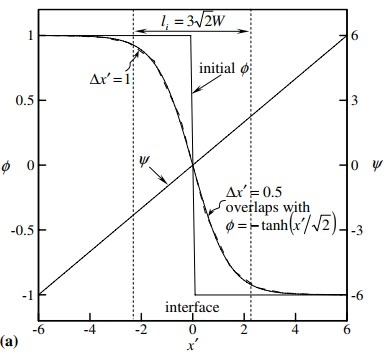
\includegraphics[width=9cm]{pf_ls.jpg}
\caption{\small Comparison of phase field variable and level set function on the interface of a stationary interface with step function like initial condition}
\label{fig:fig:pf_ls}
\end{figure}


\subsection{Evolution under constant normal speed}

For an interface with constant velocity, the Eq. \ref{eq:phase_field_final} can be simplified according to the condition of $a=\text{const.}$, $\boldsymbol{u}_{\mathrm{e}}=0$, and $b=0$ ($b$ exists in the equation as a numerical parameter for smoothing the interface):

\begin{equation}
\phi_{t}+a \frac{1-\phi^{2}}{\sqrt{2} w}=b \phi_{xx} + b\frac{f(\phi)}{w^{2}}
\end{equation}

Defining Eq. \ref{eq:dimenless_variables} variables yields to:

\begin{equation}
\frac{1}{t_c}\phi_{t^{\prime}}+\frac{a}{w} \frac{1-\phi^{2}}{\sqrt{2}}=\frac{b}{w^2} \phi_{x^{\prime}x^{\prime}} + \frac{b}{w^{2}}f(\phi)
\end{equation}
and by further reordering:

\begin{equation}
\phi_{t^{\prime}}+\frac{1-\phi^{2}}{\sqrt{2}}=b^{\prime}\left( \phi_{x^{\prime}x^{\prime}} + f(\phi)\right)
\end{equation}
with $b^{\prime}=b/aw$. For a stable numerical implementation, $\Delta t^{\prime}/\Delta x^{\prime} < 0.1$ and $b^{\prime} < 1.2$ should be met roughly.


\subsection{Curvature-driven interface evolution}

A dimensionless form of Eq. \ref{eq:phase_field_final} can be derived using a similar method for the stationary interface for a multidimensional case with $u_{\mathrm{n}}=-b\kappa$, $a=0$, and $\boldsymbol{u}_{\mathrm{e}}=0$:

\begin{equation} \label{eq:pf_curvature}
\frac{\partial \phi}{\partial t^{\prime}}=\nabla^{\prime 2} \phi+\phi\left(1-\phi^{2}\right)
\end{equation}
in which $t^{\prime}$ and $\nabla^{\prime}$ are defined similar to Eq. \ref{eq:dimenless_variables} as $t^{\prime}=t/(w^2/b)$ and $\nabla^{\prime}=\nabla/w$, respectively.

\section{Numerical implementation}

Numerical solution of the phase-field equation involves dealing with the non-linearity of the equation. Additionally, in the case of dimensional form (Eq. \ref{eq:phase_field_final}), small coefficients of the state variable in the PDE leads to numerical difficulties. As a result, numerical implementation of the phase-field equation, especially for the spectral methods such as finite element method, is still an active field of research. 

In the finite element method, the solution of a PDE is calculated based on a sum of a set of certain basis functions, which are commonly piecewise polynomial functions that are non-zero only on a small element. For doing this, the PDE is first written in a weak formulation, and then the weak form is projected on a discretized space (a set of elements) to be written as the summation of the basis functions. 

In this section, the numerical solution of the stationary form (Eq. \ref{eq:stationary_general}) and its corresponding considerations are elaborated as an example of employing the finite element formulation for simulating the phase-field equation. So, by assuming $b=1$ and $f(\phi)=\phi\left(1-\phi^{2}\right)$, the problem can be summarized as:
\begin{equation} \label{eq:fe_problem}
\left\{\begin{array}{ll}
\frac{\partial \phi}{\partial t}-\Delta \phi+\frac{1}{w^{2}} f(\phi)=0, & (x, t) \in \Omega \times(0, T] \\
\left.\frac{\partial \phi}{\partial n} \right|_{\partial \Omega}=0 \\
\left.u\right|_{t=0}=u_{0}
\end{array}\right.
\end{equation}
which demonstrates the PDE, the boundary condition, and the initial condition of the phase field variable where $\Omega$ is the domain of interest, $\partial \Omega$ is its boundary, and $T$ is the final time. Deriving the weak formulation of Eq. \ref{eq:fe_problem} is relatively straightforward as it can be seen as a time-dependent diffusion-reaction PDE, but the difficulty arises for choosing the numerical stability scheme for discretizing the temporal derivative and dealing with the non-linearity of $f(\phi)$ while normally the $\frac{1}{w^{2}}$ coefficient is a small number.

Incorporating a first-order semi-explicit scheme for Eq. \ref{eq:fe_problem} yields to:
\begin{equation} \label{eq:semi-implicit}
\frac{1}{\Delta t}\left(\phi^{n+1}-\phi^{n}, v\right)+\left(\nabla \phi^{n+1}, \nabla v\right)+\frac{1}{w^{2}}\left(f\left(\phi^{n}\right), v\right)=0, \quad \forall v \in H^{1}(\Omega)
\end{equation}
where $\Delta t$ is the time step, $(\cdot,\cdot)$ denotes the inner product, and $H^{1}(\Omega)$ is the Sobolev space of the domain $\Omega$, which is a space of functions whose derivatives are square-integrable functions in $\Omega$. The main issue with this discretization scheme is its restrictive time step condition which should satisfy:
\begin{equation}
\Delta t < \frac{2w^2}{L}
\end{equation}
where $L$ is a limit related to the non-linear part:
\begin{equation}
\max \left|f^{\prime}(\phi)\right| \leq L
\end{equation}
Obviously, as $\Delta t \sim w^2$, a very small time step is required to achieve stability in this scheme. 

Taking advantage of a fully implicit scheme improves the stability as it will be unconditionally stable, but it results to an equation that is difficult to implement as it needs solving a fixed point problem at each step. For example, a modified second-order implicit Crank-Nicolson scheme for Eq. \ref{eq:fe_problem} can be written as:
\begin{equation}
\left(\frac{\phi^{n+1}-\phi^{n}}{\Delta t}, v\right)+\left(\nabla \frac{\phi^{n+1}+\phi^{n}}{2}, \nabla v\right)+\frac{1}{w^{2}}\left(\tilde{f}\left(\phi^{n+1}, \phi^{n}\right), v\right)=0, \quad \forall v \in H^{1}
\end{equation}
where:
\begin{equation}
\tilde{f}(u, v)=\left\{\begin{array}{ll}
\frac{F(u)-F(v)}{u-v} & \text { if } u \neq v \\
f(u) & \text { if } u=v
\end{array}\right.
\end{equation}
in which $F$ is the potential term ($f(\phi)=F^{\prime}(\phi)$).

An alternative can be deriving a stabilized semi-implicit scheme by adding a stabilization term to Eq. \ref{eq:semi-implicit}. A first-order version of such a scheme can be written as:
\begin{equation}
\left(\frac{1}{\Delta t}+\frac{S}{w^{2}}\right)\left(\phi^{n+1}-\phi^{n}, v\right)+\left(\nabla \phi^{n+1}, \nabla v\right)+\frac{1}{w^{2}}\left(f\left(\phi^{n}\right), v\right)=0, \quad \forall v \in H^{1}(\Omega)
\end{equation}
which is unconditionally stable for every $S \geq \frac{L}{2}$.

\section{Adapting the formulation for  curvature-driven tissue growth}

In order to adapt Eq. \ref{eq:pf_curvature} for the curvature-driven process of neo-tissue growth, one can consider the following equation:
\begin{equation} \label{eq:pf_tissue}
\frac{\partial \phi}{\partial t^{\prime}}=\left(\nabla^{\prime 2} \phi+\phi\left(1-\phi^{2}\right)\right).H\left(\nabla^{\prime 2} \phi+\phi\left(1-\phi^{2}\right)>0\right)
\end{equation}
in which $H$ denotes a heaviside step function. Eq. \ref{eq:pf_tissue} implies that the growth is only allowed for regions with a positive curvature (right hand side of Eqs. \ref{eq:phase_field_final} and \ref{eq:pf_curvature}).

Using the same approach, a similar level set formulation can be obtained based on Eq. \ref{eq:ls_general} by omitting the normal velocity and curvature terms and embedding the effect of the curvature in the velocity field. Doing this yields to a convection equation for the distance function:
\begin{equation} \label{eq:ls_advect}
\frac{\partial \psi}{\partial t}+\boldsymbol{u} \cdot \nabla \psi=0,
\end{equation}
in which the convection velocity field can be defined as:
\begin{equation} \label{eq:ls_veloc}
\boldsymbol{u}=\left\{\begin{array}{ll}
-\kappa \boldsymbol{n} & \text { if } \kappa>0 \\
0 & \text { if } \kappa \leq 0
\end{array}\right.
\end{equation}
with $\kappa$ being calculated similar to Eq. \ref{eq:curvature} for a distance function $\psi$. In practical implementations, the distance function is not differentiable at every location of the domain due to discontinuities in the gradients, so one can consider taking advantage of artificial diffusion terms to overcome this issue, leading to the following equations for the normal vector and curvature calculation:
\begin{equation}
\boldsymbol{n}=\frac{\nabla \varphi}{|\nabla \varphi|}+\varepsilon \Delta \boldsymbol{n}
\end{equation}
\begin{equation}
\kappa=\nabla \cdot \boldsymbol{n}+\varepsilon \Delta \kappa
\end{equation}
in which $\epsilon$ denotes the numerical diffusion coefficient.


\begin{subappendices}

\section{Implementing the phase-field model using physics-informed neural networks}



\end{subappendices}

%%%%%%%%%%%%%%%%%%%%%%%%%%%%%%%%%%%%%%%%%%%%%%%%%%
% Keep the following \cleardoublepage at the end of this file, 
% otherwise \includeonly includes empty pages.
\cleardoublepage

